\section{Introduction}

\begin{frame}{Décomposition de Helmholtz--Hodge}
\begin{figure}[H]
    \centering
    \def\imgw{0.2\textwidth}
\def\sep{1.7cm}
\def\buf{1.3cm}

\begin{tikzpicture}
\node at (0*\sep,0) {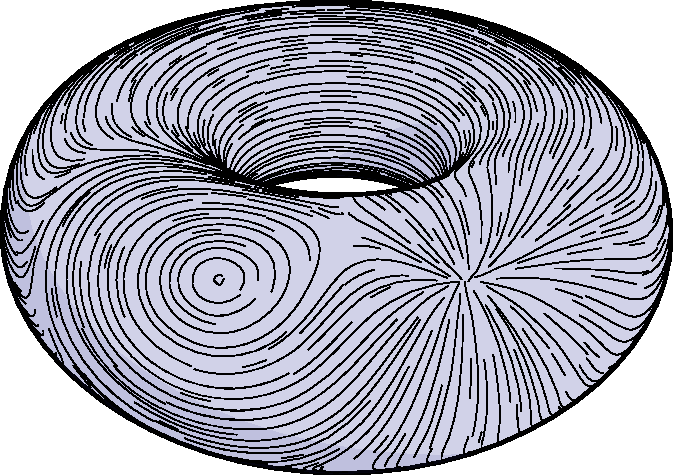
\includegraphics[width=\imgw]{img/input.pdf}};
\node at (1*\sep,0) {\Large $=$};
\node at (2*\sep,0) {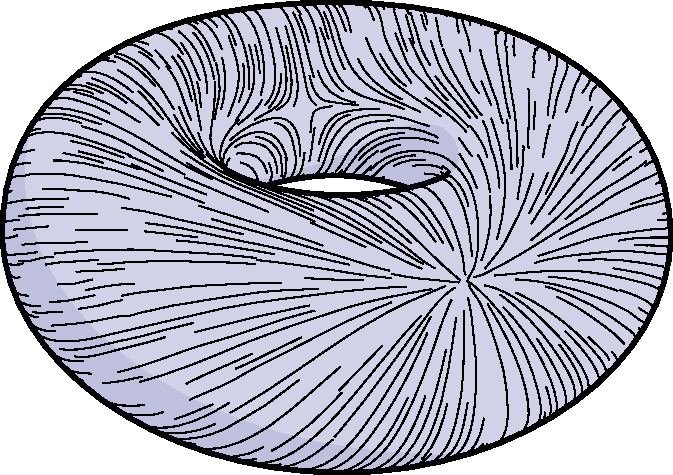
\includegraphics[width=\imgw]{img/grad.pdf}};
\node at (3*\sep,0) {\Large $+$};
\node at (4*\sep,0) {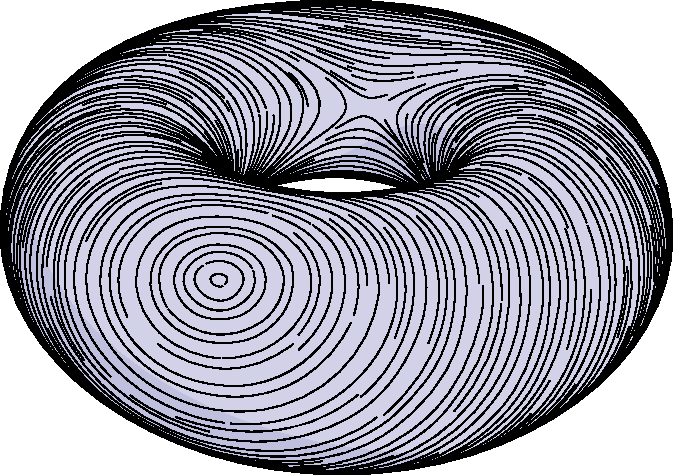
\includegraphics[width=\imgw]{img/rot.pdf}};
\node at (5*\sep,0) {\Large $+$};
\node at (6*\sep,0) {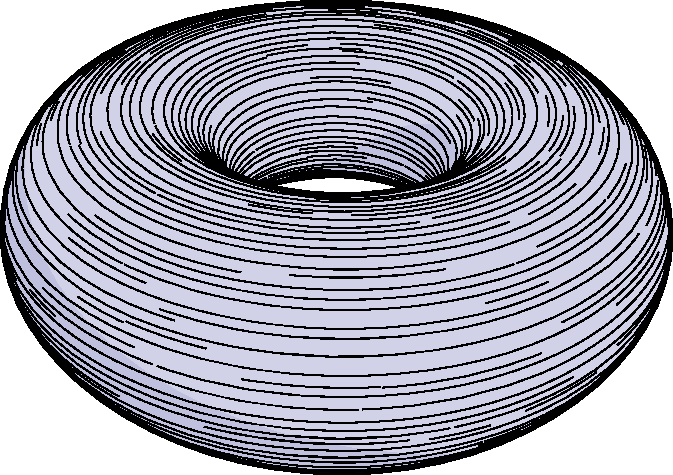
\includegraphics[width=\imgw]{img/harmo.pdf}};

\node at (0*\sep,\buf) {$\vect{\xi}$};
\node at (2*\sep,\buf) {$\grad \phi$};
\node at (2*\sep,-\buf) {irrotationnel};
\node at (4*\sep,\buf) {$\rot \psi$};
\node at (4*\sep,-\buf) {solénoïdal};
\node at (6*\sep,\buf) {$\vect{h}$};
\node at (6*\sep,-\buf) {harmonique};
\end{tikzpicture}
\end{figure}

\begin{itemize}
    \item Liens avec les \sftxt{équations de Maxwell} sous leur formulation en potentiels
\end{itemize}
\end{frame}

\begin{frame}{Méthodes de volumes finis}
\begin{exampleblock}{Avantages}
\begin{itemize}    
    \item Font appel à des bilans locaux (de masse, d'énergie, \dots)
    \item Sens physique très concret
    \item Grande robustesse
    \item Maillages très généraux
\end{itemize}
\end{exampleblock}
\begin{alertblock}{Inconvénients}
\begin{itemize}
    \item Définir les flux sur la frontière des volumes de contrôle
    \item Difficile à appliquer aux maillages non structurés / non conformes
\end{itemize}
\end{alertblock}

\begin{center}
\stxt{$\implies$ Méthode \ddfv}
\end{center}

\end{frame}

\begin{frame}{Méthode \emph{Discrete Duality Finite Volume} (\ddfv)}
\framesubtitle{Classe des méthodes de volumes finis à \textbf{grilles décalées}}

\begin{columns}[c]
\begin{column}{0.6\textwidth}
\begin{itemize}
    \item<1-> {\color{myblue} Maillage primal $\ensprimalplat$}
    \item<2-> {\color{myred} Maillage dual $\ensdualplat$}
    \item<3-> {\color{mydarkgreen} Maillage diamant $\ensdiamantplat$}
\end{itemize}
\medskip
\begin{itemize}
    \item<2-> Inconnues scalaires sur $\ensddfvplat = ({\color{myblue}\ensprimalplat}, {\color{myred}\ensdualplat})$
    \item<3-> Inconnues vectorielles sur ${\color{mydarkgreen}\ensdiamantplat}$
\end{itemize}
\end{column}
\begin{column}{0.4\textwidth}
\begin{figure}
    \centering
    \input{figures_beamer/ddfv.tex}
\end{figure}
\end{column}
\end{columns}
\onslide<4->{
\begin{boite}{myblue}
\begin{center}
Discrétisation des gradients dans \textbf{toutes les directions} \\
Conservation des propriétés des opérateurs au \textbf{niveau discret}
\end{center}
\end{boite}
}
\bigskip
\onslide<5->{
\[
\size(\ensddfvplat) \defeq \max_{E \in {\color{myblue}\ensprimalplat} \cup {\color{myred}\ensdualplat} \cup {\color{mydarkgreen}\ensdiamantplat}} \mathrm{diam}(E)
\qquad
\reg(\ensddfvplat) \defeq 
\begin{matrix}
    \text{«\,mesure applatissement et rapport} \\
    \text{entre les tailles des mailles\,»}
\end{matrix}
\]
\begin{center}
$\reg(\ensddfvplat)$ \stxt{uniformément borné} lorsque $\size(\ensddfvplat) \to 0$.     
\end{center}
}
\end{frame}

\begin{frame}
\begin{envide}[Objectif : Théorème d’approximation]
\textsl{Soit $(\ensddfvplat_n)_n$ des maillages t.q. $\size(\ensddfvplat_n) \xrightarrow[n \to \infty]{} 0$ et $\reg(\ensddfvplat_n)$ borné $\forall n \in \N$ :
\vspace{-0.2cm}
\[
\forall \vect{\xi} \in (\L^2(\surflisse))^2,
\quad
(\phi^{\ensddfvplat_n}, \psi^{\ensddfvplat_n}, h^{\ensdiamantplat_n})
\xrightarrow[n \to \infty]{\L^2}
(\phi, \psi, \vect{h}).
\]
}
\end{envide}

\begin{block}{Programme}
\begin{enumerate}
    \only<1>{\item \fauxhighlighttxt{Généralisation de la méthode \ddfv sur les surfaces fermées de $\R^3$}}
    \only<1>{\item \fauxhighlighttxt{Inégalité de Poincaré discrète}}
    \only<2->{\item \highlighttxt{Généralisation de la méthode \ddfv sur les surfaces fermées de $\R^3$}}
    \only<2->{\item \highlighttxt{Inégalité de Poincaré discrète}}
    \item Théorème de type Riesz--Fréchet--Kolmogorov
    \item Théorème de compacité discrète
\end{enumerate}
\end{block}
\begin{overprint}[\textwidth]
\only<3>{
\vspace{-0.15cm}
\begin{block}{État de l'art}
\begin{itemize}
    \item \cit{Omnes \emph{et al.}, '05, '07} : \ddfv pour des domaines à bord dans $\R^2$
    \item \cit{Andreianov, Boyer, Hubert, '07} : Inégalité de Poincaré \ddfv dans $\R^2$
    \item Inégalité de Poincaré : aucune démonstration pour les surfaces fermées de $\R^3$
    \item Convergence numérique de la méthode \ddfv sur la sphère
    \item \cit{Tomek, Mikula \emph{et al.}, '16, '19} : expériences numériques \ddfv pour le problème surfacique de flot de courbure moyenne
\end{itemize}
\end{block}
}
\onslide<4->{
\begin{columns}
\begin{column}{0.5\textwidth}
\begin{alertblock}{Difficultés sur les surfaces sans bord}
\begin{itemize}
    \item Absence de bord au domaine
    \item En 2D : $\surfpoly \subset \surflisse$, en 3D : $\surfpoly \not\subset \surflisse$
\end{itemize}
\end{alertblock}
\end{column}
\begin{column}{0.5\textwidth}
    \centering
    \begin{tikzpicture}[
    every path/.style={thick,line join=round, cap=round},
]

\tdplotsetmaincoords{45}{55}

\node[visible on=<1>] at (3,1.5) {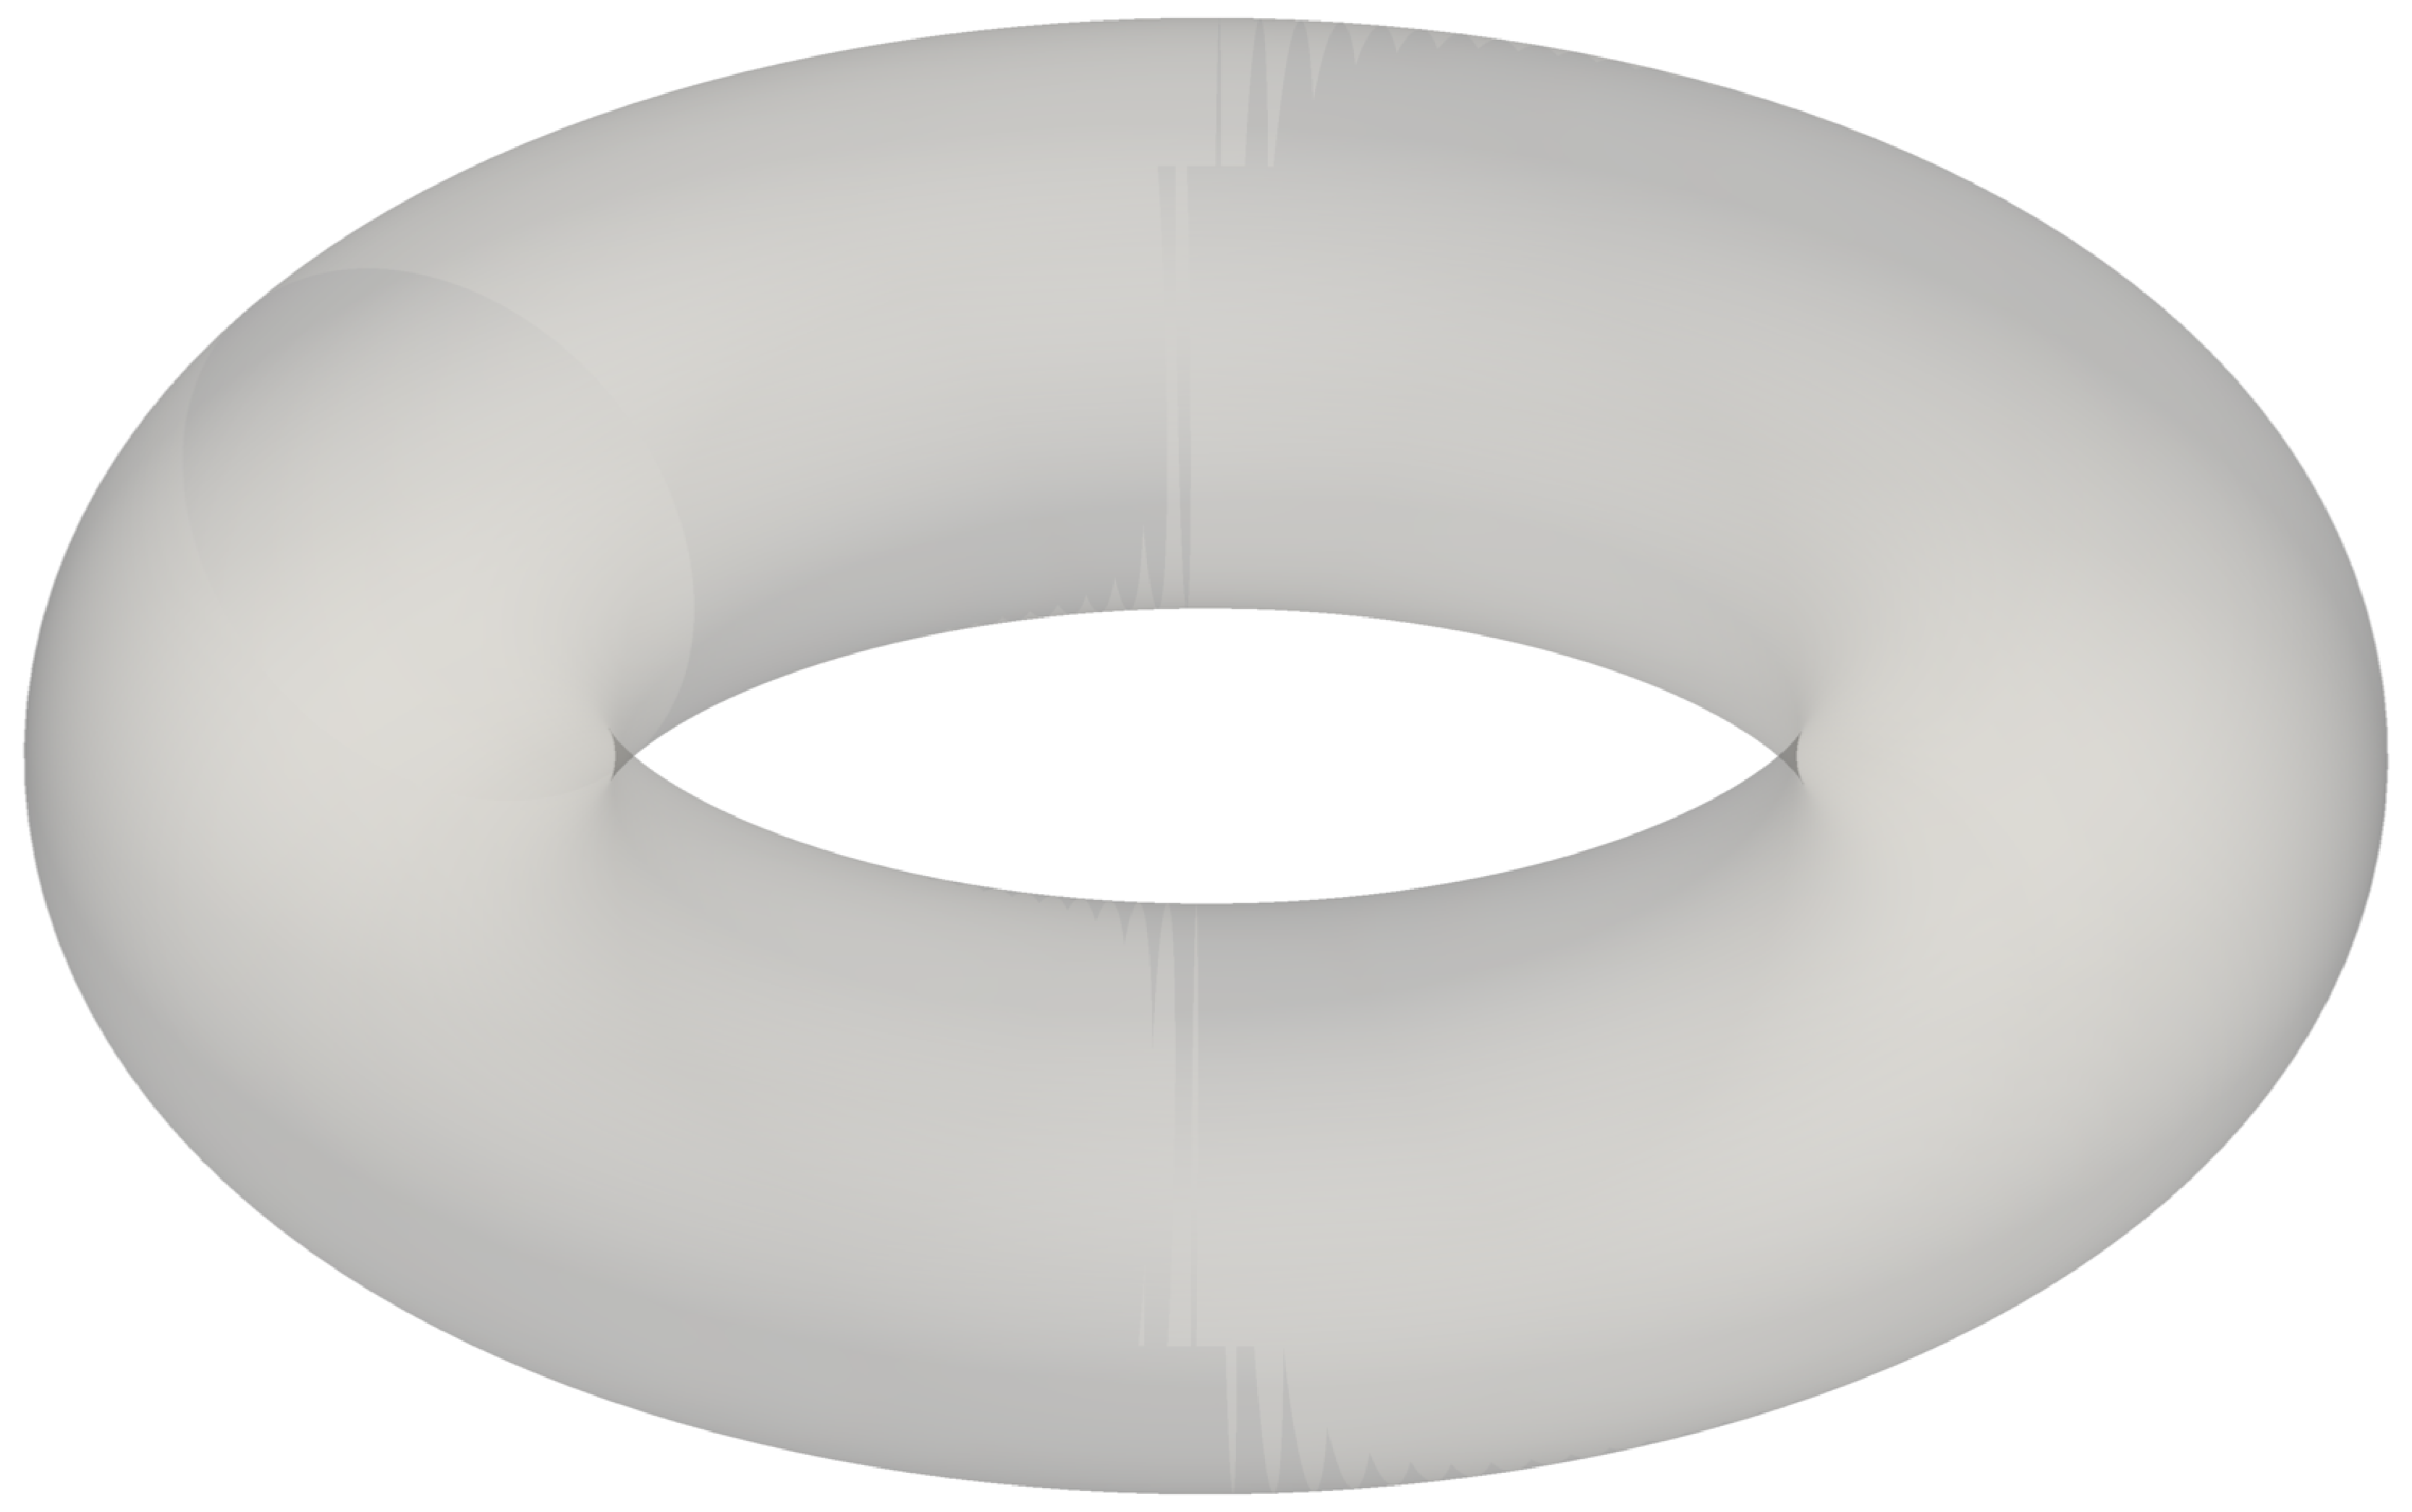
\includegraphics[width=0.9\textwidth]{img/torus_lisse.pdf}};
\node[visible on=<1->] (torepoly) at (3,1.5) {%
    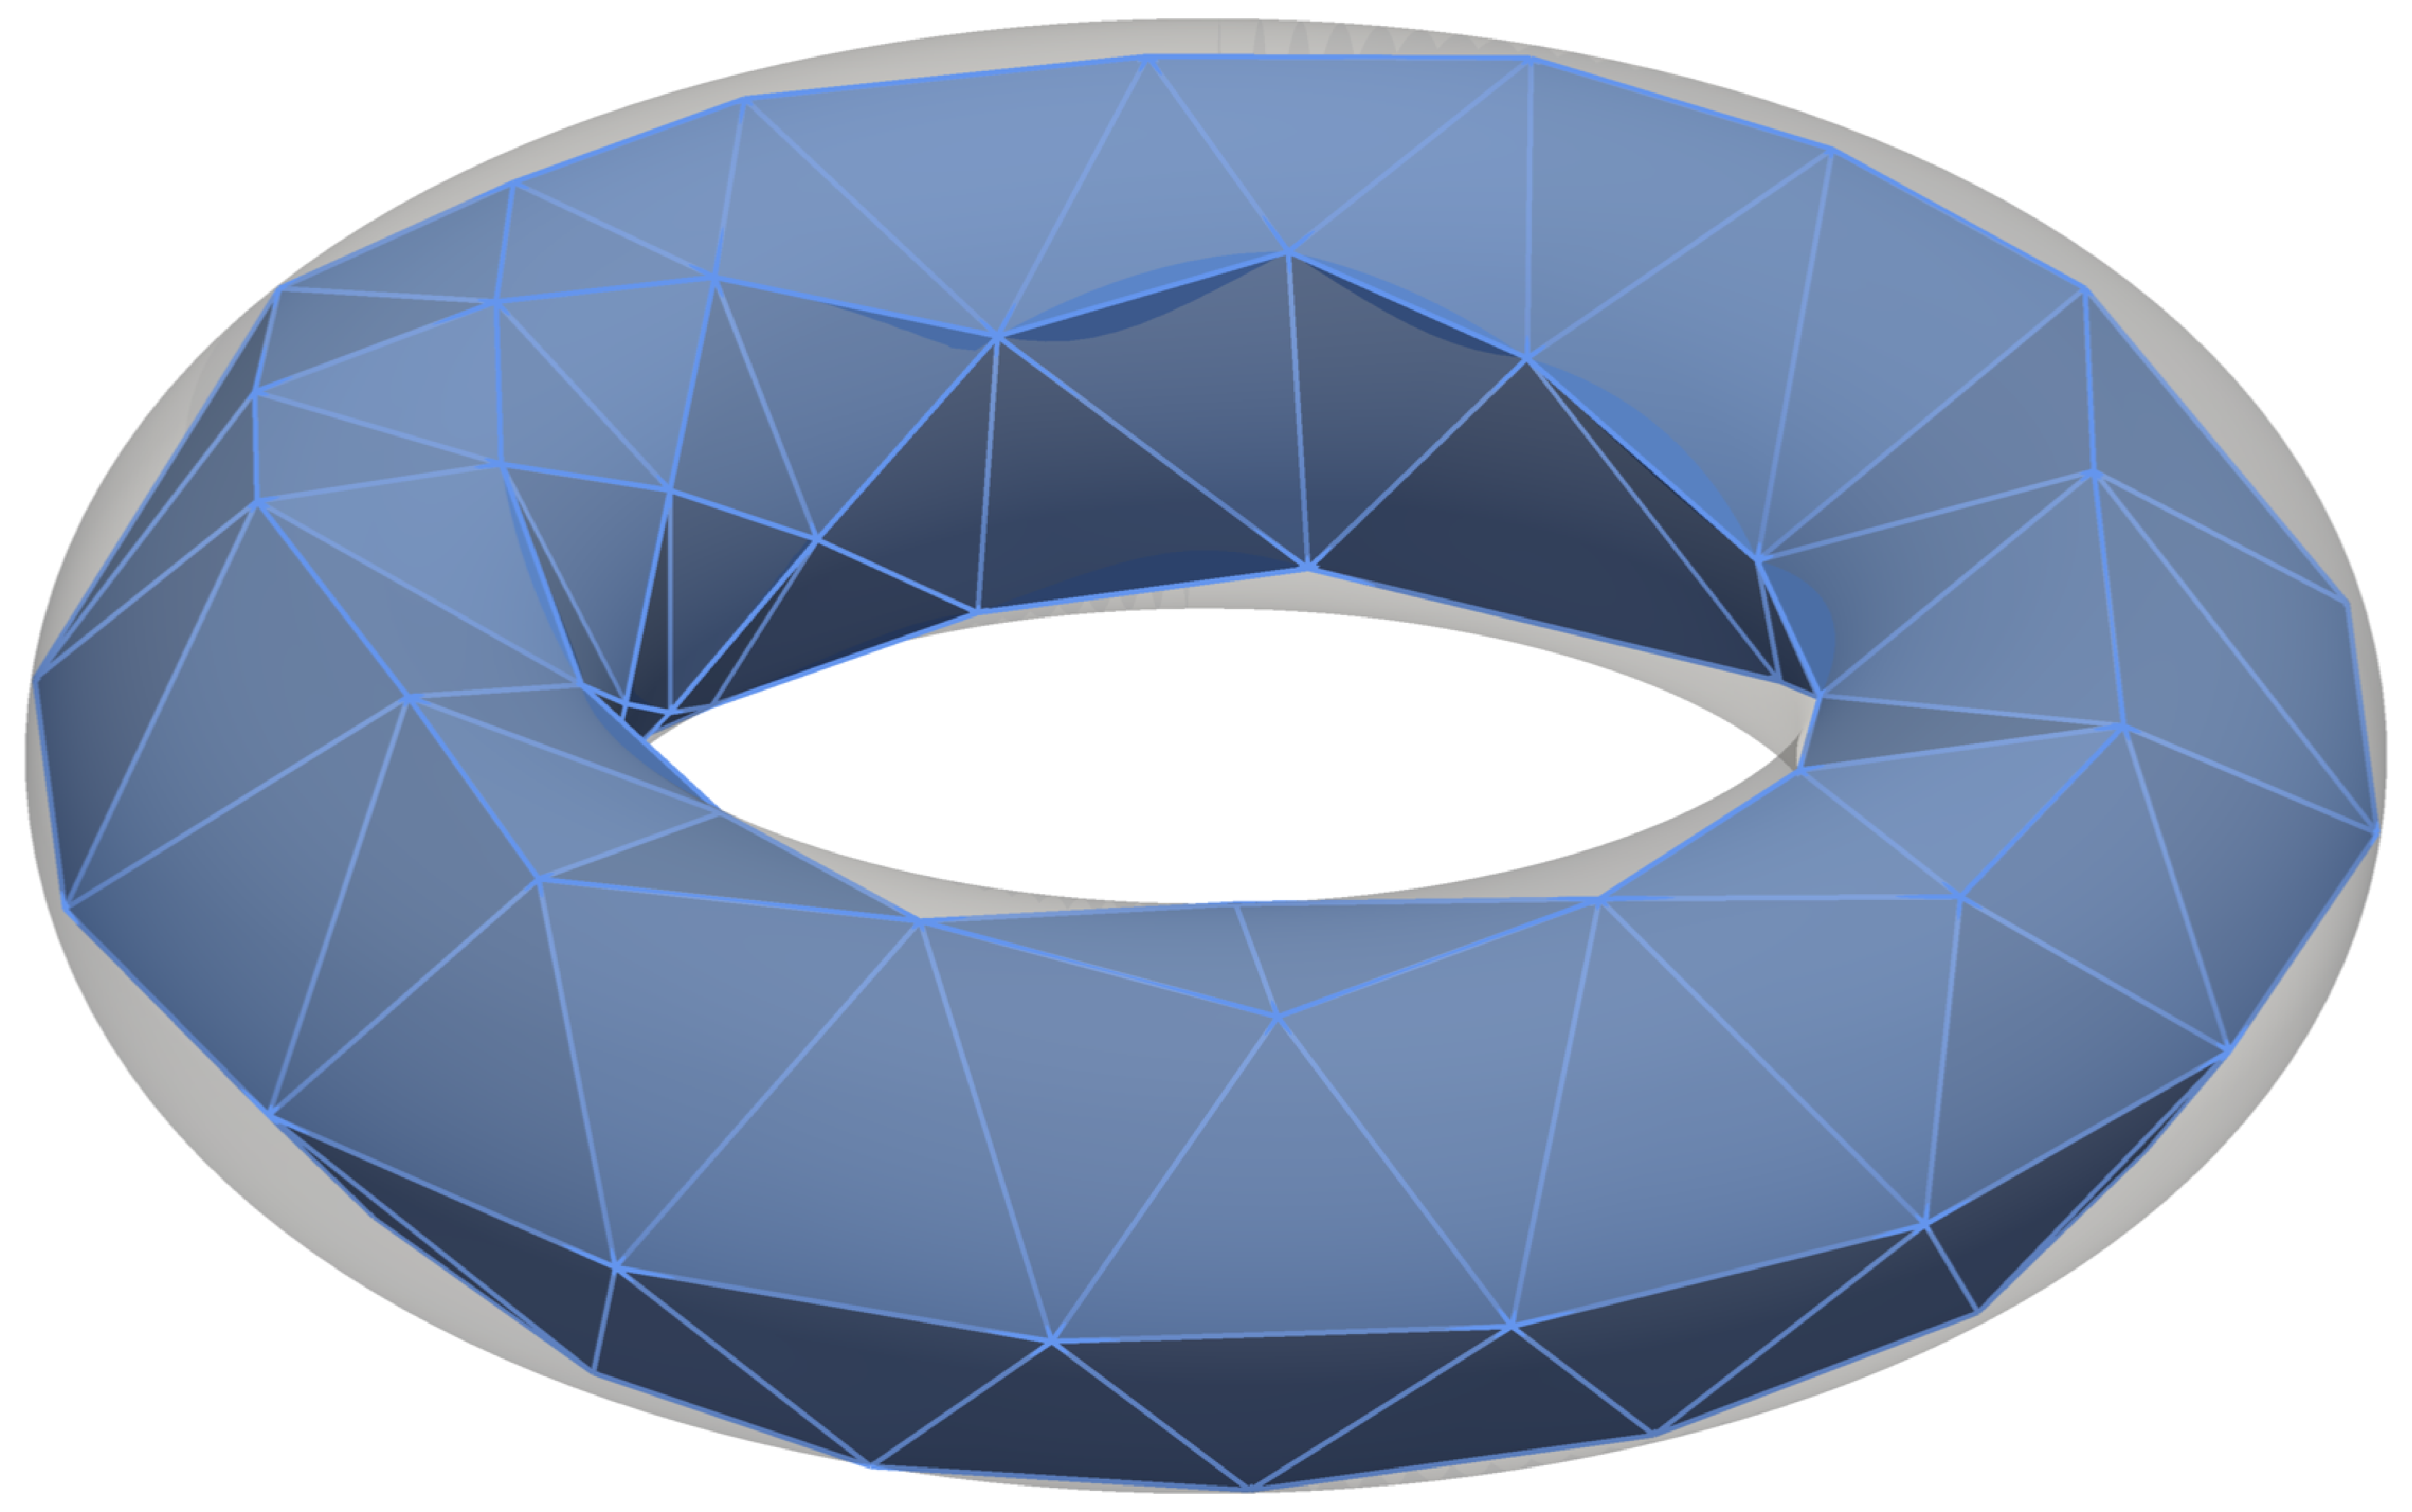
\includegraphics[width=0.9\textwidth]
    {img/torus_lisse_et_primal.pdf}%
};

% \node[visible on=<1->, above] at (torepoly.north) {\highlight{\surfpoly \not\subset \surflisse}};

\end{tikzpicture}

\end{column}
\end{columns}
}
\end{overprint}
\end{frame}